\section{Билет 3. Задача Коши для уравнения колебаний струны. Формула Даламбера. Область зависимости решения от начальных данных. Существование и единственность классического решения. Корректность постановки задачи}
% Затехал: Рязанов Андрей
\textbullet\ Задача $\begin{cases} u_{tt}-a^2u_{xx} = 0\\ \while{u(t,x)}{t=0} = u_0(x)\\ \while{u_t}{t=0} = u_1(x)\end{cases}\quad -l<x<l$\\
Что понимать под решением задачи?\\
\begin{definition}[Классическое решение]
{\bf Классическое решение} -- функция класса $C^2$, которая в точках указанной области удовлетворяет уравнению и заданным соотношениям.\\
\end{definition}
\textbullet\ {\bf Характеристическое уравнение: } $(dx)^2 - a^2(dt)^2 = 0$\\
$\begin{cases} \xi = x+at \\ \eta = x-at \end{cases} \Leftarrow \begin{cases} x+at = C_1 \\ x-at = C_2 \end{cases}$\\
В новых координатах $\hat{u}_{\xi\eta}(\xi,\eta) = 0\ \To \hat{u} = f(\xi) + g(\eta) $.\\
Возвращаясь обратно, получим $u(t,x) = f(x+at) + g(x-at)$.\par
\textbullet\ Решим ЗК (поверхности нигде не касаются характеристик -- задача должна быть корректной):
\begin{equation*}
\begin{aligned}
&\while{u}{t=0} = u(0,x) = f(x) + g(x) = u_0(x), \quad &-l < x< l&\\
&\while{u_t}{t=0} =  af'(x) - ag'(x) = u_1(x), \quad &-l < x< l& \quad \To\ f(x) - g(x) = \frac1{a}\int _{-l}^xu_1(z)dz + C = \frac1{a}V_1(x)
\end{aligned}
\end{equation*}
\begin{center}
$\Downarrow$
\end{center}
\begin{equation}
\label{eq::3::dalam}
\tag{*}
\begin{cases} f(x) = \frac1{2}u_0(x) + \frac1{2a}V_1(x) \\ g(x) = \frac1{2}u_0(x) - \frac1{2a}V_1(x) \end{cases} \quad (-l < x< l)
\end{equation}
\[ u(t,x) = \frac1{2}u_0(x+at) + \frac1{2a}V_1(x+at) + \frac1{2}u_0(x-at) - \frac1{2a}V_1(x-at) =\]\[= \boxed{\frac{u_0(x+at) + u_0(x-at)}{2} + \frac1{2a}\int_{x-at}^{x+at}u_1(x)dx} - \text{{\bf формула Даламбера}} \]
Решение определяется единственным образом.\par
Если требуется определить максимальную область, где можно написать решение, то обратимся к формулам \eqref{eq::3::dalam}. Функции $u_0$ и $V$ определены лишь на $(-l;l)\ \To\ $искомая область: $\begin{cases} -l<x+at<l \\ -l<x-at<l\end{cases}$ -- {\bf характеристический четырехугольник $Q$}.\par\bigskip
\begin{wrapfigure}{r}{0.25\textwidth}
%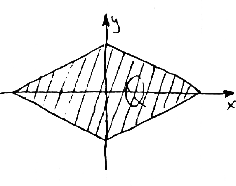
\includegraphics[width=0.9\linewidth]{3_1_new} 
%\begin{comment}
\begin{tikzpicture}[scale = 0.5]
  \tikzstyle{axes}=[]
  \tikzstyle{important line}=[very thick]
  \tikzstyle{information text}=[rounded corners,fill=red!10,inner sep=1ex]

   \begin{scope}[style=axes]
    \draw[->] (-4,0) -- (4,0) node[right] {$x$};
    \draw[->] (0,-3) -- (0,3) node[left] {$y$};
    \end{scope}

    \coordinate (A) at (0, -2);
    \coordinate (B) at (3, 0);
    \coordinate (C) at (0, 2);
    \coordinate (D) at (-3, 0);
    \draw[pattern = north east lines, pattern color = blue] (A) -- (B) -- (C) -- (D) -- cycle;

    \coordinate [label = {right: \LARGE $Q$}] (F) at (1, 0);
    \end{tikzpicture}
%\end{comment}
\end{wrapfigure}
Нами доказана теорема:
\begin{theorem}
Пусть $\begin{cases} u_0(x)\in C^2(-l;l) \\ u_1(x) \in C^1(-l;l) \end{cases}$. Тогда ЗК имеет в $Q$ единственное решение $u(t,x)\in C^2(Q)$ -- классическое. Оно дается формулой Даламбера.
\end{theorem}
\par

\textbullet\ Корректность задачи для уравнения малых колебаний струны:
\begin{itemize}
\item нами проверены существование и единственность классического решения.
\item покажем непрерывность решения по входным данным $u_0$ и $u_1$.\\Берем две задачи:
\[ \begin{cases} \stackrel{\text{\tiny{1}}}{u}_{tt}-a^2\stackrel{\text{\tiny{1}}}{u}_{xx} = 0, \quad (t,x)\in Q\\ 
\while{\stackrel{\text{\tiny{1}}}{u}}{t=0} = \stackrel{\text{\tiny{1}}}{u}_0(x), \quad \abs{x}<l\\ \while{\stackrel{\text{\tiny{1}}}{u}_t}{t=0} = \stackrel{\text{\tiny{1}}}{u}_1(x), \quad \abs{x}<l\end{cases} \qquad
\begin{cases} \stackrel{\text{\tiny{2}}}{u}_{tt}-a^2\stackrel{\text{\tiny{2}}}{u}_{xx} = 0, \quad (t,x)\in Q\\
\while{\stackrel{\text{\tiny{2}}}{u}}{t=0} = \stackrel{\text{\tiny{2}}}{u}_0(x), \quad \abs{x}<l\\
\while{\stackrel{\text{\tiny{2}}}{u}_t}{t=0} = \stackrel{\text{\tiny{2}}}{u}_1(x), \quad \abs{x}<l\end{cases}
\]
Пусть $\abs{\stackrel{\text{\tiny{1}}}{u}_0 - \stackrel{\text{\tiny{2}}}{u}_0}<\delta_0,\ \abs{\stackrel{\text{\tiny{1}}}{u}_1 - \stackrel{\text{\tiny{2}}}{u}_1}<\delta_1\quad \forall x:\ \abs{x}<l.$ Введем 
$\begin{cases}
v_0 = \stackrel{\text{\tiny{1}}}{u}_0 - \stackrel{\text{\tiny{2}}}{u}_0 \\
v_1 = \stackrel{\text{\tiny{1}}}{u}_1 - \stackrel{\text{\tiny{2}}}{u}_1 \\
v = \stackrel{\text{\tiny{1}}}{u} - \stackrel{\text{\tiny{2}}}{u}
\end{cases}$\\
Тогда задача для $v:\ \begin{cases} 
v_{tt}-a^2v_{xx} = 0, \quad (t,x) \in Q\\ 
\while{v}{t=0} = v_0(x),\quad \abs{x}<l,\ \abs{v_0}<\delta_0\\ 
\while{v_t}{t=0} = v_1(x),\quad \abs{x}<l,\ \abs{v_1}<\delta_1
\end{cases}$.\\
Согласно формуле Даламбера, $\abs{v(t,x)} = \abs{\dfrac{v_0(x+at) + v_0(x-at)}{2} + \dfrac1{2a}\int\limits_{x-at}^{x+at}v_1(y)dy} \le \delta_0 + \delta_1t \quad \forall (t,x) \in Q.$
\begin{itemize}
\item[--] Если $l$ конечно, то $t\le \dfrac{l}{a}$ из вида четырёхугольника $Q$. Устремляя $\delta_0, \delta_1 \to 0$, получим $\abs{v}\to 0$.
\item[--] Если $l=\infty$: в любой конечной полосе $t\le T< \infty$ требуемое верно. \\
Так заметаем всю плоскость.


\end{itemize}
\end{itemize}
